\subsection{Algoritmi di stima}
Il sistema robotico preso in esame presenta degli errori all'ingresso degli
encoder, tale errore porta il sistema a manifestare nel lungo periodo il noto
comportamento di \emph{drift}.
Nasce allora il problema di correggere e stimare la posizione in base ad un dato
modello.
Stimando la posizione del robot utilizzando la ricostruzione odometrica si
ottiene un risultato affetto da incertezza crescente all'aumentare dello
spostamento.
È necessario quindi correggere tale stima attraverso il particle
filter\cite{newman2003} analizzato di seguito.
Ciò su cui ci appoggeremo per avere una stima della posizione assunta dal robot,
saranno dei sensori esterni ad esso, nel nostro caso delle ancore \textsc{Wi-Fi}
virtualmente simulate.

\subsubsection{Filtro Particellare}
L'algoritmo di localizzazione PF procede come segue in figura
\ref{fig:particle filter}. Si inizializzano $n$ particelle in una mappa.
Ogni particella è un vettore di stato $q\,=\,[x \, y \, \theta]^{T}$ del veicolo
ed ad ognuna di queste si applica il modello descritto dal sistema di 
eq.(\ref{eq:modelcinematico}): e se ne aggiunge un rumore al vettore di
controllo $u\,=\,[v \, \omega]^{T}$.
Successivamente per ogni particella si prevede la possibile misura ottenibile e
si confronta con l'osservazione realmente effettuata dalla ancora
\textsc{Wi-Fi}, tale confronto porterà al calcolo dell'innovazione o di ciò che
definiremo peso della particella.
Si selezionano le particelle che meglio spiegano l'osservazione, un modo per
farlo è quello di costruire una pdf che descriva i campioni e i loro pesi, e
poi riselezionare un nuovo set di particelle da questa pdf.
La stima della posizione del robot fornita dal filtro è la media di questo
nuovo ricampionamento.
Il punto cruciale è che non richiede alcuna ipotesi di linearizzazione (non ci
sono jacobiani coinvolti) e non ci sono ipotesi Gaussiane. È particolarmente
adatto ai problemi con piccoli spazi di stato mentre in caso di vettori di
stato grandi diventa computazionalmente pesante.

\begin{figure}[!htb]
 \centering
  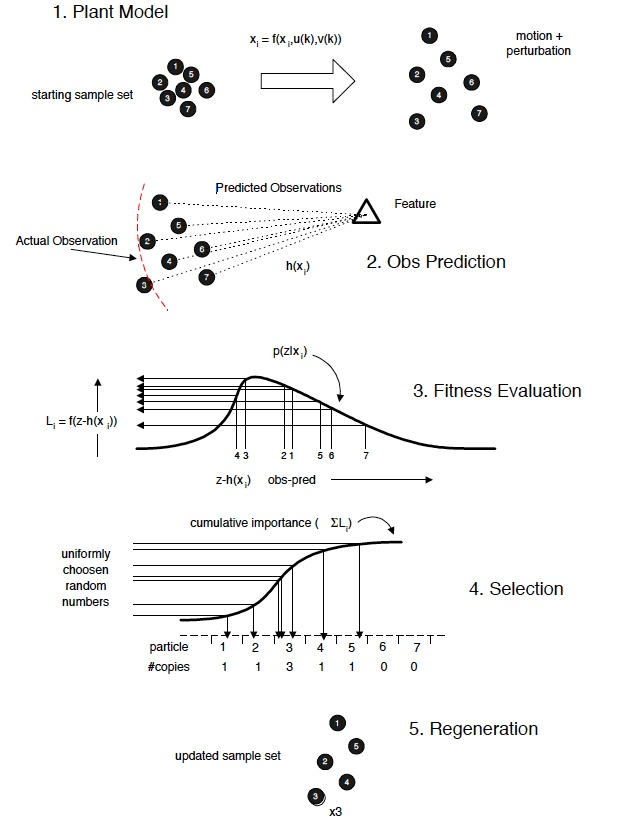
\includegraphics[width=.4\textwidth]{particle_filter}
  \caption{Filtro Particellare}
  \label{fig:particle filter}
\end{figure}
